% Chapter Template

\chapter{Temporal Coherent Backmapping of Molecular Trajectories} % Main chapter title

MD simulations evolve a molecular system in time and allow to track its path in phase space. The obtained trajectory is a set of states compatible with the starting condition, i.e. samples drawn from the accessible area in phase space. Typically, consecutive frames of the trajectory are separated by a fixed time step, which controls the correlation between recorded frames. Computing time averages over a trajectory yields structural or thermodynamic properties, such as the radial distribution function or energies. However, the temporal information stored in the trajectory allows to compute dynamic properties as well. In particular, time correlations can be used to link simulation results to experimental observables. Examples include (1) the diffusion constant, which can be computed as the integral of the velocity auto-correlation,\cite{frenkel2001understanding} (2) (infrared) absorption spectra, which is related to the auto-correlation function of the total dipole moment \cite{bergsma1984electronic, guillot1991molecular} and (3) scattering functions that can be related to Fourier transforms of the van Hove correlation function.\cite{PhysRevE.53.2382, moe1999calculation} Note that some important dynamic properties, such as the dynamic structure factor, require atomistic details in order to allow a comparison with experimental data.\cite{chen2008comparison, arbe2012neutron} However, while time correlation functions are central to the analysis of dynamic properties, typical reverse-mapping strategies are frame-based, i.e. each molecular snapshot of the trajectory is treated separately. Such backmapping schemes are not temporally aware and the correlations between consecutive frames are only maintained via large-scale characteristics. Consequently, reintroduced degrees of freedom between consecutive frames might decorrelate locally. As such, time correlation functions based on local, atomistic descriptors are typically not reliable for such backmapped trajectories. 

\begin{figure}
  \centering
      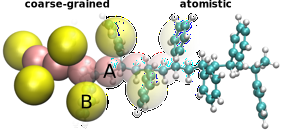
\includegraphics[width=0.5\textwidth]{./Figures/temporal_coherent_bm/intro.pdf}
  \caption{asfafasf}
  \label{FIG:TEMP_COH_intro}
\end{figure}


In this chapter, a new method to perform temporally coherent backmapping of molecular simulation trajectories is introduced. The proposed method aims at both, generating well-equilibrated molecular structures for each frame and achieve temporal coherence within a series of frames. To this end, a ML model is deployed that reconstructs a molecular structure in one-shot leveraging configurational information from previous simulation frames. In particular, the model is conditioned on the current coarse- and previous fine-grained configurations (see Fig. \ref{FIG:TEMP_COH_intro}). In contrast to the previously deployed GAN-based method DBM, a conditional variational autoencoder (CVAE) is used for this task. 

The method is demonstrated for two biomolecular systems: Alanine dipeptide (ADP) and the miniprotein chignolin (CLN). In addition to in-distribution testing, i.e. reconstructing a coarse-grained atomistic trajectory similar to the training data, the trained model is also deployed for trajectories obtained with a coarse-grained simulation. Specifically, the coarse-grained forcefield generated by a ML-based method CGSchnet is used in both cases.\cite{} The performance of the model is evaluated in terms of reconstructed energetic, thermodynamic and kinetic properties.

The work presented in this chapter stems from a collaboration with Kirill Shmillovich, Moritz Hoffmann and Nick Charron. The project originates from the long program \textit{Machine Learning for Physics and the Physics of Learning} at the Institute for Pure \& Applied Mathematics that was held from  09.04.19 to 12.08.19 at the University of California, Los Angeles. 

\section{Method}

The proposed method is similar in spirit to the previously used method DBM, but differs in some major aspects: (1) Molecules are considered in vacuum and not in the condensed-phase. As such, representations and the backmapping protocol can be simplified. (2) The ML model $g_{\Theta}$ generates all the atoms of a molecular configuration in one shot, i.e. not autoregressively. To this end, coarse-grained and atomistic representations fed to the model have to capture the molecular structure in its whole extend. In particular, atoms and beads are represented as smooth densities $\gamma$ and $\Gamma$ (Eq. \ref{DBM:density_representation}) expressed on a discretized grid due to voxelization, as outlined in Sec. \ref{DBM:representation}. Note that the center of mass is removed for each molecule in order to ensure that each molecule is fully enclosed by the grid representation. To avoid clutter, each particle is placed in its own feature channel, i.e. a molecule containing $N$ particles with positions $\mathbf{r} \in \mathbb{R}^{3N}$ is represented as a four-dimensional tensor $\varepsilon(\mathbf{r}) \in \mathbb{R}^{N \times s \times s \times s}$, where $s$ is the grid size. (3) The input arguments for the model $g_{\Theta}$ consist of the current coarse-grained frame $\mathcal{E}(\mathbf{R}_{t}) \in \mathbb{R}^{N \times s \times s \times s}$ and previous reconstructed fine-grained frame $\varepsilon(\mathbf{\hat{r}}_{t - \tau}) \in \mathbb{R}^{N \times s \times s \times s}$, where $\mathbf{R} \in \mathbb{R}^{3N}$ and $\mathbf{\hat{r}} \in \mathbb{R}^{3n}$ denote the coordinates of the $N$ coarse-grained beads and $n$ reconstructed atoms, respectively, $t$ is the current time and $\tau$ is the time step between consecutive frames. In addition, a sample $\mathbf{z} \in \mathbb{R}^{d}$ of the latent distribution $\mathcal{Z}$ is incorporated as source of randomness. (4) The ML model is trained end-to-end using a variational autoencoder architecture (Sec. \ref{}) instead of the generative adversarial approach. In particular, latent samples $\mathbf{\hat{z}}$ are generated by an encoder network $e_{\Psi}$. The encoder $e_{\Psi}\big( \varepsilon(\mathbf{\hat{r}}_{t}), \varepsilon(\mathbf{\hat{r}}_{t - \tau}), \mathcal{E}(\mathbf{R}_{t}) \big)$ is a function of the current atomistic frame $\varepsilon(\mathbf{\hat{r}}_{t})$, previous atomistic frame $\varepsilon(\mathbf{\hat{r}}_{t - \tau})$ and the current coarse-grained frame $\mathcal{E}(\mathbf{R}_{t})$. As such, training of the model is based on the reconstruction of a given atomistic frame, i.e. $\varepsilon(\mathbf{r}_{t})$, and does not rely on an critic network. In particular, the deployed cost-function $\mathcal{C}$ is constructed as

\begin{align}
    \mathcal{C} &= \mathcal{C}_{\text{recon vox}} + \mathcal{C}_{\text{recon pos}} + \mathcal{C}_{\text{CG}} + \mathcal{C}_{\text{EDM}} + \lambda  \mathcal{C}_{\text{energy}} + \beta \mathcal{C}_{\text{KL}} \label{eqn:loss} \\
    \mathcal{C}_{\text{recon vox}}(\mathbf{r}_t, \hat{\varepsilon}) &= \frac{1}{s^3n}\ || \varepsilon(\mathbf{r}_{t}) - \hat{\varepsilon} ||_2^2  \notag \\
    \mathcal{C}_{\text{recon pos}}(\mathbf{r}_t, \mathbf{\hat{r}}_t) &= \frac{1}{3n}\ || \mathbf{r}_{t} - \mathbf{\hat{r}}_{t} ||_2^2 \notag \\
    \mathcal{C}_{\text{CG}}(\mathbf{R}_t, \mathbf{\hat{r}}_t) &= \frac{1}{3N}\ || \mathbf{R}_t - M(\mathbf{\hat{r}}_t) ||_2^2 \notag \\
    \mathcal{C}_{\text{EDM}}(\mathbf{r}_t, \mathbf{\hat{r}}_t) &= \frac{1}{2n^2}\ || EDM(\mathbf{r}_{t}) - EDM(\mathbf{\hat{r}}_{t}) ||_2^2 \notag \\
    \mathcal{C}_{\text{energy}}(\mathbf{r}_t, \mathbf{\hat{r}}_t) &= (U(\mathbf{{r}_{t}}) - U(\mathbf{\hat{r}}_{t}))^2 \notag \\
    \mathcal{C}_{\text{KL}}(\mathbf{\hat{z}}) &= \mathcal{D}_{KL}(\mathbf{\hat{z}}||\mathcal{N}(0,\mathbf{I})). \notag ,
\end{align}

where $\varepsilon{\hat{r}} = g_{\Theta}(\varepsilon(\mathbf{\hat{r}}_{t - \tau}), \mathcal{E}(\mathbf{R}_{t}, \mathbf{\hat{z}})$ is the density prediction by the decoder, and $\mathbf{\hat{r}}$ denotes collapsed coordinates (see Sec. \ref{DBM:cGAN}). The first four terms in Eq. \ref{eqn:loss} can be associated with reconstruction. In particular, $\mathcal{C}_{\text{recon vox}}$ denotes the reconstruction loss for the spatially voxelized particle densities representations and $\mathcal{C}_{\text{recon pos}}$ is the reconstruction loss in terms of the coordinates. Moreover, the coarse-grained mapping function $M$ is deployed in $\mathcal{C}_{\text{CG}}$ in order to enforce consistency between the input coarse-grained structure $\mathbf{R}$ and the coarse-grained backmapped configuration $M(\mathbf{\hat{r}})$. Furthermore, $\mathcal{C}_{\text{EDM}}(\mathbf{r}_t, \mathbf{\hat{r}}_t)$ computes the mean squared error between the Euclidean Distance Matrices (EDM) of the target configuration $\mathbf{r}$ and reconstructed configuration $\mathbf{\hat{r}}$. As such, $\mathcal{C}_{\text{EDM}}(\mathbf{r}_t, \mathbf{\hat{r}}_t)$ aims at recovering inter-particle distances correctly. In addition, the atomistic force field is deployed in $\mathcal{C}_{\text{energy}}(\mathbf{r}_t, \mathbf{\hat{r}}_t)$ to calculate the mean squared error of the potential energies for the target structure $\mathbf{r}$ and reconstruction $\mathbf{\hat{r}}$. $\mathcal{C}_{\text{energy}}(\mathbf{r}_t, \mathbf{\hat{r}}_t)$ serves as a regularizer to improve the quality of backmapped structures, which might suffer from resolution limits of the voxel representation. As such, it accelerates convergence and helps more precisely match the reconstructed energetics to the ground truth trajectory. Since the potential energy is sensitive to small pertubations of the coordinates, it can become dominatingly large during the early stages of training before the model learns to stably localize atomic coordinates. To alleviate this issue, the prefactor $\lambda$ is incorporated which is set to $\lambda = 0$ at the beginning of the training and slowly annealed up to $\lambda = 1$ using an exponential annealing schedule. Beside reconstruction terms, $\mathcal{C}_{\text{KL}}(\mathbf{\hat{z}})$ acts as a regularization term to bias the approximate posterior $\mathbf{\hat{z}} = e_{\Psi}\big( \varepsilon(\mathbf{\hat{r}}_{t}), \varepsilon(\mathbf{\hat{r}}_{t - \tau}), \mathcal{E}(\mathbf{R}_{t}) \big)$ towards the desired prior distribution, i.e. a normal distribution $\mathcal{N}(0,\mathbf{I})$. The associated prefactor $\beta$ scales the regularization loss and is set to $\beta = 1$ for the CLN model, while a cyclic annealing schedule for $\beta$ is deployed to mitigate KL vanishing.\cite{}

While the encoder $e_{\Psi}$ is indispensable during training in order to implement the reconstruction loss, it is omitted at inference time and the latent sample $\mathbf{z}$ is drawn from a prior distribution. Specifically, $\mathbf{z}$ is drawn from a Gaussian Mixture Model fitted to the latent distribution implied by the encoder, instead of the assumed prior $p(\mathbf{z}) \sim \mathcal{N}(\mathbf{0}, \mathbf{I})$. This process ensures that the decoder operates within densely sampled latent space regions. The actual reverse-mapping of the coarse-grained trajectory $(\mathbf{R}_0, \mathbf{R}_{\tau}, \mathbf{R}_{2\tau}, \dots )$ is performed solely by the decoder. To this end, the decoder hallucinates the atomistic trajectory autoregressively, i.e. the previous reconstructed atomistic frame $\mathbf{\hat{r}}_{t-\tau}$ serves as input for the next step at time $t$. The seed for the hallucination, i.e. the initial atomistic frame at $t=0$, is chosen from a presampled pool of atomistic configurations. In particular, a frame is chosen that has a minimal RMSD to the initial coarse-grained frame when it is mapped to coarse-grained coordinates. 

\label{temp_coherent_bm} % Change X to a consecutive number; for referencing this chapter elsewhere, use \ref{ChapterX}

\section{ADP}


\begin{figure}[H]
  \centering
      \includegraphics[width=1.0\textwidth]{./Figures/temporal_coherent_bm/ADP_fes.pdf}
  \caption{Free energy landscape }
  \label{FIG:morph_sps_free_energy}
\end{figure}

\begin{figure}[H]
  \centering
      \includegraphics[width=1.0\textwidth]{./Figures/temporal_coherent_bm/ADP_kinetics.pdf}
  \caption{Free energy landscape }
  \label{FIG:morph_sps_free_energy}
\end{figure}

\section{CLN}


\begin{figure}[H]
  \centering
      \includegraphics[width=1.0\textwidth]{./Figures/temporal_coherent_bm/CLN_fes.pdf}
  \caption{Free energy landscape }
  \label{FIG:morph_sps_free_energy}
\end{figure}

\begin{figure}[H]
  \centering
      \includegraphics[width=1.0\textwidth]{./Figures/temporal_coherent_bm/CLN_kinetics.pdf}
  \caption{Free energy landscape }
  \label{FIG:morph_sps_free_energy}
\end{figure}
